\documentclass[12pt]{article}
\usepackage{amsmath}
\usepackage{amssymb}
\usepackage{graphicx}
\usepackage{hyperref}
\usepackage{geometry}
\usepackage{float}
\geometry{a4paper, margin=1in}

\title{Intro to AI \\ Homework Assignment 1}
\author{Nikita Zagainov DSAI-01}
\date{\today}

\begin{document}

\maketitle

\section{Environment}
The environment used for testing has the following characteristics:
\begin{itemize}
    \item Deterministic (no randomness);
    \item Sequential (agent's position is defined by a sequence of previous steps);
    \item Partially observable (agent can only see the immediate surroundings);
    \item Discrete (agent can only move in four directions);
    \item Dynamic (picking backdoor key changes map);
    \item Single-agent (Enemies do not satisfy agent's properties);
    \item Known (We know all of the rules of the environment);
\end{itemize}
\section{Implementation Details}
\subsection{A Star Algorithm}
The code submitted to the assignment is an implementation of Agent that uses A*
algorithm to find best path to the goal. The implementation uses Dijkstra's
algorithm to traverse the map, the heuristic function is implemented as
Manhattan distance between the current position and the keymaker position. No
modifications were introduced to the A* algorithm in the implementation.

\subsection{Backtracking Algorithm}
The code submitted to the assignment is an implementation of Agent that uses
backtracking algorithm to find best path to the goal. The implementation uses
BFS to traverse the map considering known threats, and whenever new information
is available on dangers on built path, the agent backtracks to the last known
safe position and rebuilds the path to the goal. No significant modifications
were made to the backtracking algorithm.

\subsection{Agent Behavior}
In both implementations, agent is aiming to find the shortest path to the
keymaker, ignoring backdoor key (for simplicity), and avoiding threats. A*
agent uses A* for finding best path to the keymaker, Backtracking agent uses
BFS algorithm with backtracing on running into a threat for finding best path
to the keymaker.

\subsection{Code}
\href{https://github.com/V1adych/itai_assignment_1}{Link to the code repository}

\section{Evaluation results}
The agents were evaluated on 1000 randomly generated maps below is the summary
of the results:
\begin{table}[H]
    \centering
    \begin{tabular}{|c|c|c|}
        \hline
        \textbf{Metric}                           & \textbf{A* Algorithm} & \textbf{Backtracking Algorithm} \\ \hline
        Mean Execution Time (s)                   & 0.009                 & 0.005                           \\ \hline
        Std Execution Time (s)                    & 0.028                 & 0.013                           \\ \hline
        Var Execution Time (s\textsuperscript{2}) & 0.00079               & 0.00018                         \\ \hline
        Mean Moves                                & 9.82                  & 10.221                          \\ \hline
        Std Moves                                 & 6.085                 & 6.095                           \\ \hline
        Var Moves                                 & 37.03                 & 37.14                           \\ \hline
        Win Fraction                              & 0.881                 & 0.909                           \\ \hline
    \end{tabular}
    \caption{Evaluation results of A* and Backtracking algorithms}
    \label{tab:evaluation_results}
\end{table}
\noindent
As can be seen from the table, the algorithms do not have a big
statistical difference in terms of mean moves. However, the execution time of the A* algorithm implementation provided is slightly higher than the execution time of the backtracking algorithm, and the win fraction difference is also not very high.

\section{Unsolvable map example}
\begin{figure}[H]
    \centering
    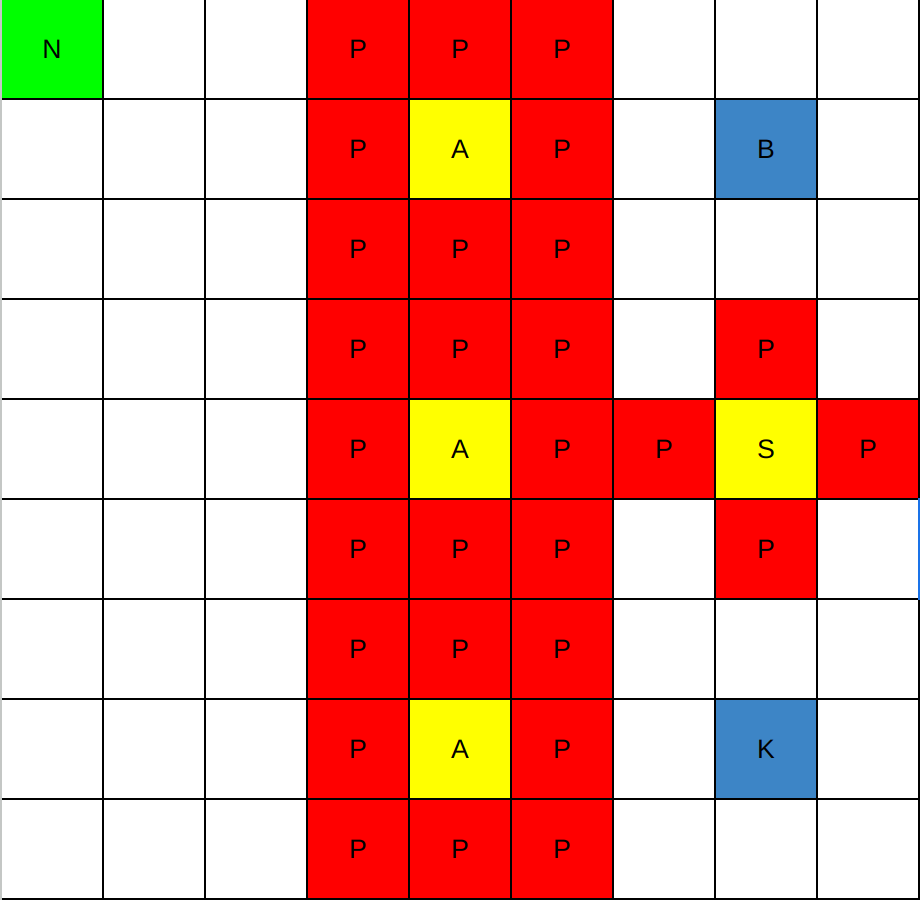
\includegraphics[width=0.8\textwidth]{unsolvable_map.png}
    \caption{Example of an unsolvable map}
    \label{fig:unsolvable_map}
\end{figure}

\subsection{Unsolvable Maps Analysis}
During the evaluation, some maps were found to be unsolvable by both A* and
Backtracking agents. These maps typically contained isolated sections or
completely blocked paths that made it impossible for the agents to reach the
keymaker. The primary reasons for unsolvability included:

\begin{itemize}
    \item Completely blocked paths with no possible route to the goal.
    \item Maps where the keymaker was surrounded by threats with no safe path available.
\end{itemize}
\noindent
The example shown in Figure \ref{fig:unsolvable_map} illustrates a scenario where the path to the keymaker and backdoor key is completely blocked, making it impossible for the agent to find a solution.
\section{Conclusion}
This assignment solution provides two implementations of the agent that can
solve the problem of path finding. Both algorithms were implemented without any
modifications. The evaluation results show that the backtracking algorithm has
slightly better performance in terms of execution time, but both algorithms
show approximately the same performance in terms of mean moves and win
fraction.
\end{document}
